\chapter{ISTTOK }

ISTTOK is a large aspect ratio tokamak (IPFN-IST, Lisbon, Portugal) operating since 1990 and which has been in constant upgrading of diagnostics, hardware acquisition system and control algorithms (major and minor plasma radius are respectively $R= 46 \, cm$, $a= 8.5 \, cm$). Together with the JT60-SA development of control techniques from last chapter, ISTTOK  studies  complement as a whole this work. This chapter will detailed how ISTTOK operates, from topics such as describing its diagnostics to description of the reconstruction method for calculating the plasma centroid position.

\section{Machine description}
The construction  of the actual ISTTOK machine was started in mid-1990 reusing some parts of the former dutch TORTUT tokamak: support structure, vacuum vessel, copper shell, toroidal magnetic coils, transformer, capacitor banks, radiofrequency (rf) generator, and discharge cleaning system ~\cite{Varandas1996}. The other components of ISTTOK such as the vacuum systems, the poloidal windings, and the power supply for the toroidal magnetic coils,  as well as its diagnostics and control and data acquisition system, were locally designed and built. Figure ~\ref{TopISTTOK} shows a top view of the ISTTOK tokamak and figure~\ref{ISTTOK_front} a frontal one in early 2020, its main elements are signalized with arrows.\smallskip

\begin{figure}[htbp]
	\centering
	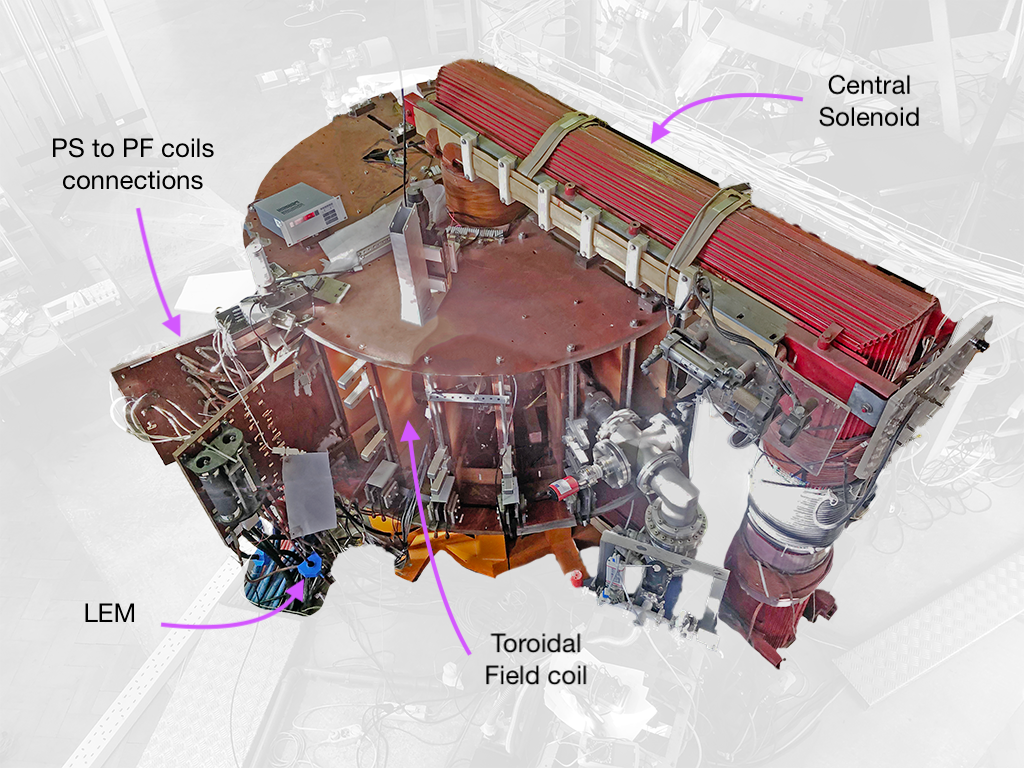
\includegraphics[width=0.95\textwidth]{Chp4/TopISTTOK.png}
	\caption{\label{TopISTTOK} ISTTOK top view in 2020,   main elements are indicated with magenta  lines.}
\end{figure}

\begin{figure}[htbp]
	\centering
	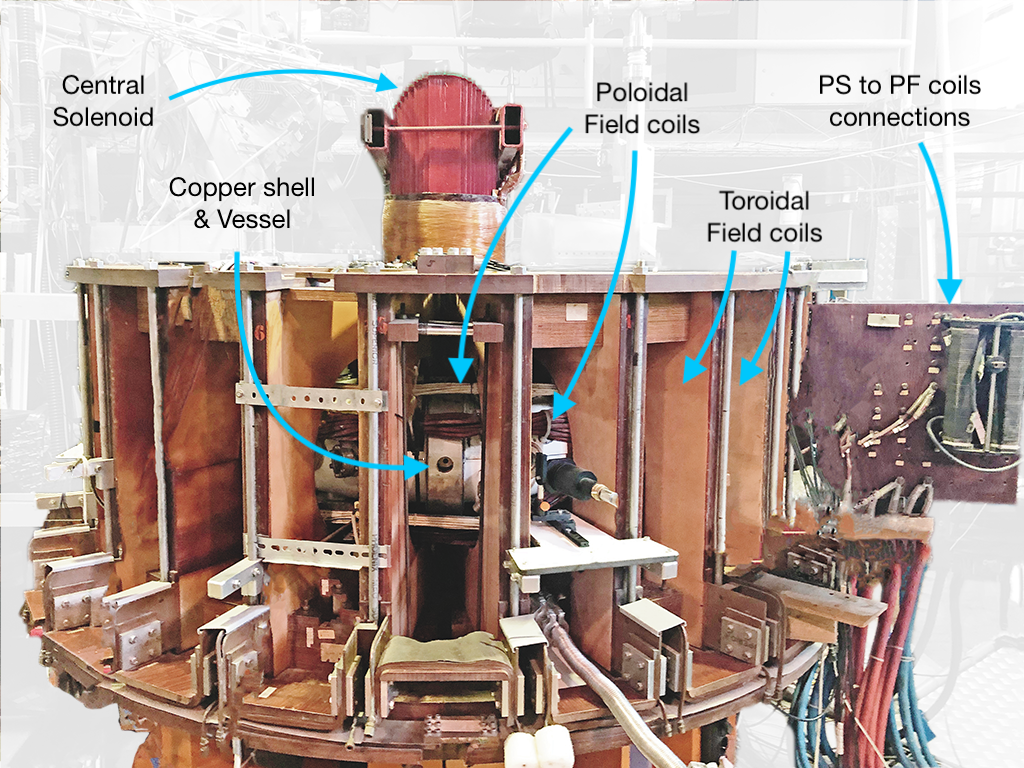
\includegraphics[width=0.95\textwidth]{Chp4/FrontISTTOK.png}
	\caption{\label{ISTTOK_front}ISTTOK frontal view in 2020, main elements are indicated with blue lines.   }
\end{figure}

Figure ~\ref{VV_IST} corresponds to a section of the ISTTOK vacuum vessel, it is possible to observe on the image the ribbed  surface from the vessel and some of the ports on the top of it.

\begin{figure}[htbp]
	\centering
	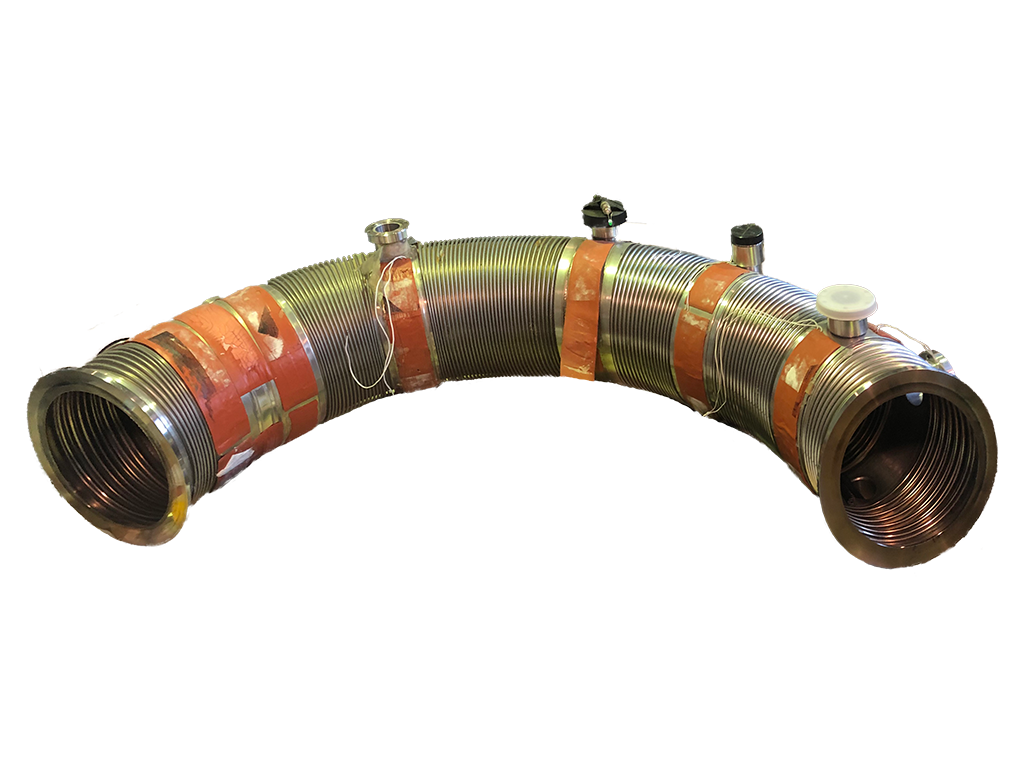
\includegraphics[width=0.65\textwidth]{Chp4/VacuumVessel_Low.png}
	\caption{\label{VV_IST} Actual ISTTOK inconel  vaccum vessel section with ports.  }
\end{figure}






\section{Diagnostics and Actuators}

\begin{figure}[htbp]
	\centering
	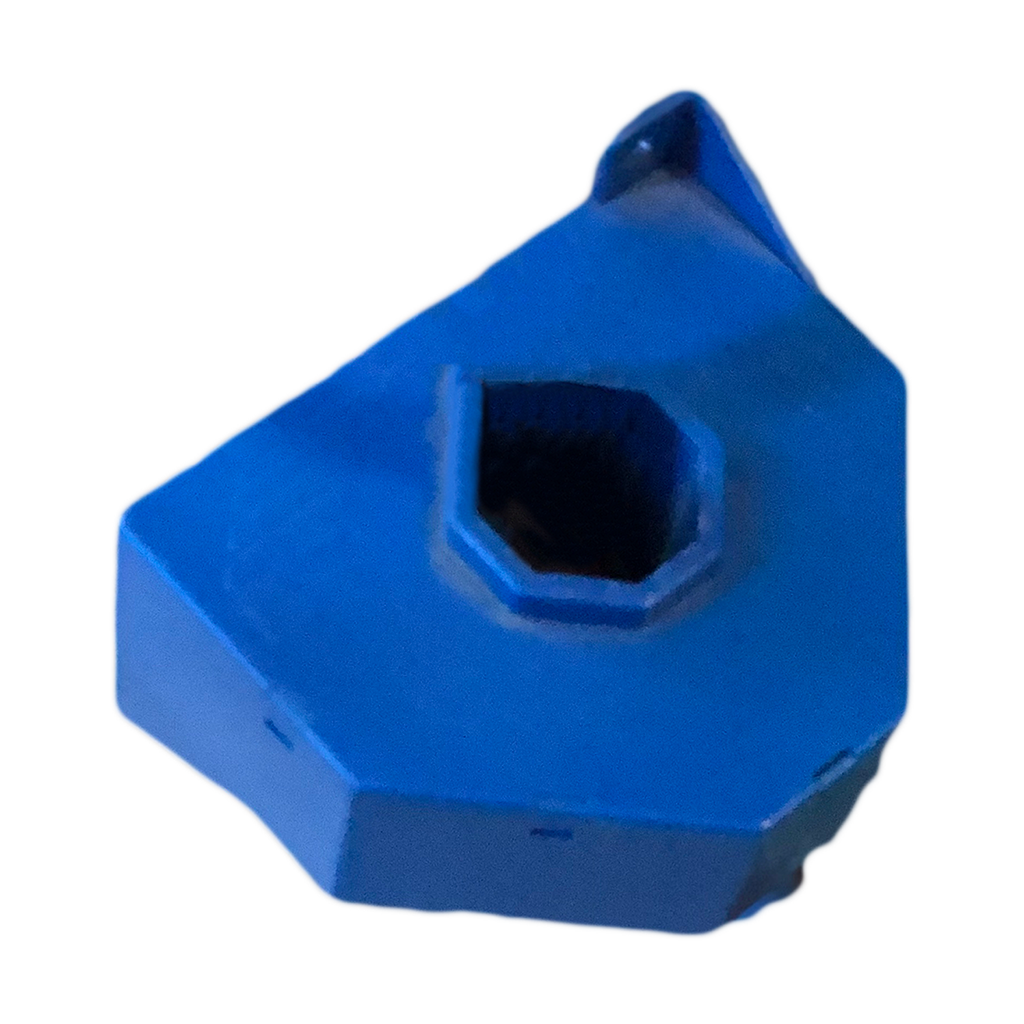
\includegraphics[width=0.4\textwidth]{Chp4/LEM.png}
	\caption{\label{LEM} LEM transducer for measuring the current from the PS to the PF coils.  }
\end{figure}

\begin{figure}
	\centering
	\begin{subfigure}[b]{0.37\textwidth}
		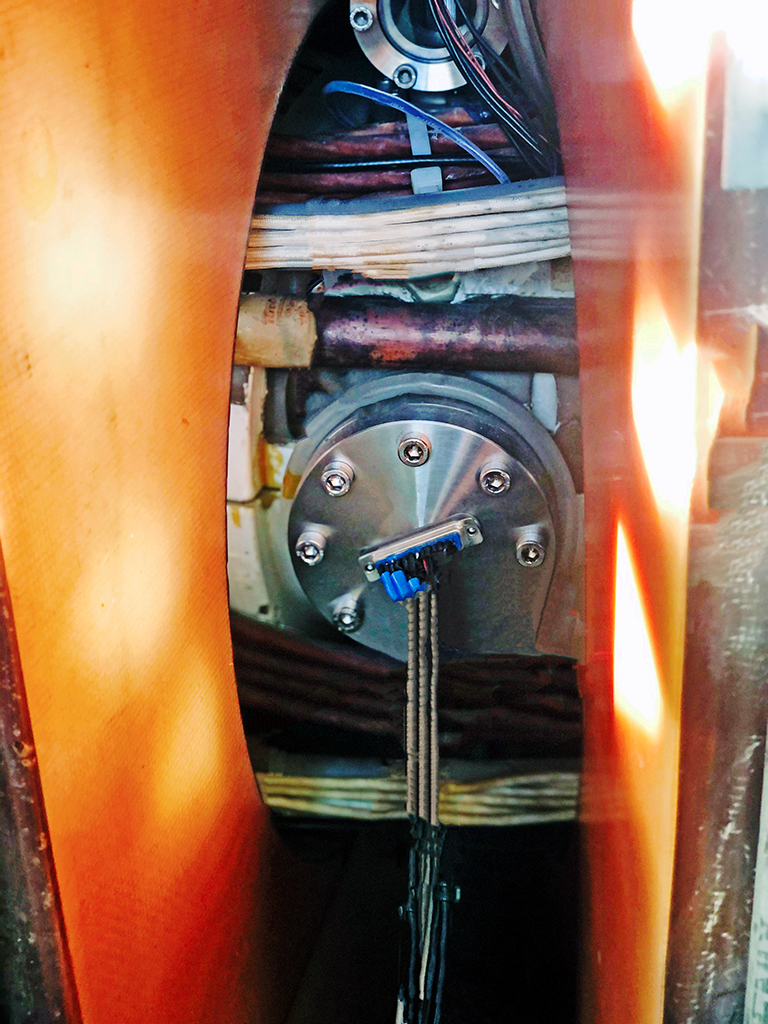
\includegraphics[width=\textwidth]{Chp4/PuertoMirnov.png}
	\caption{\label{MirnPort}Magnetic probes port with connection cable to the ATCA acquisition boards, also PF coils and cooper shell are shown. }
	\end{subfigure}
~~~~
	\begin{subfigure}[b]{0.37\textwidth}
		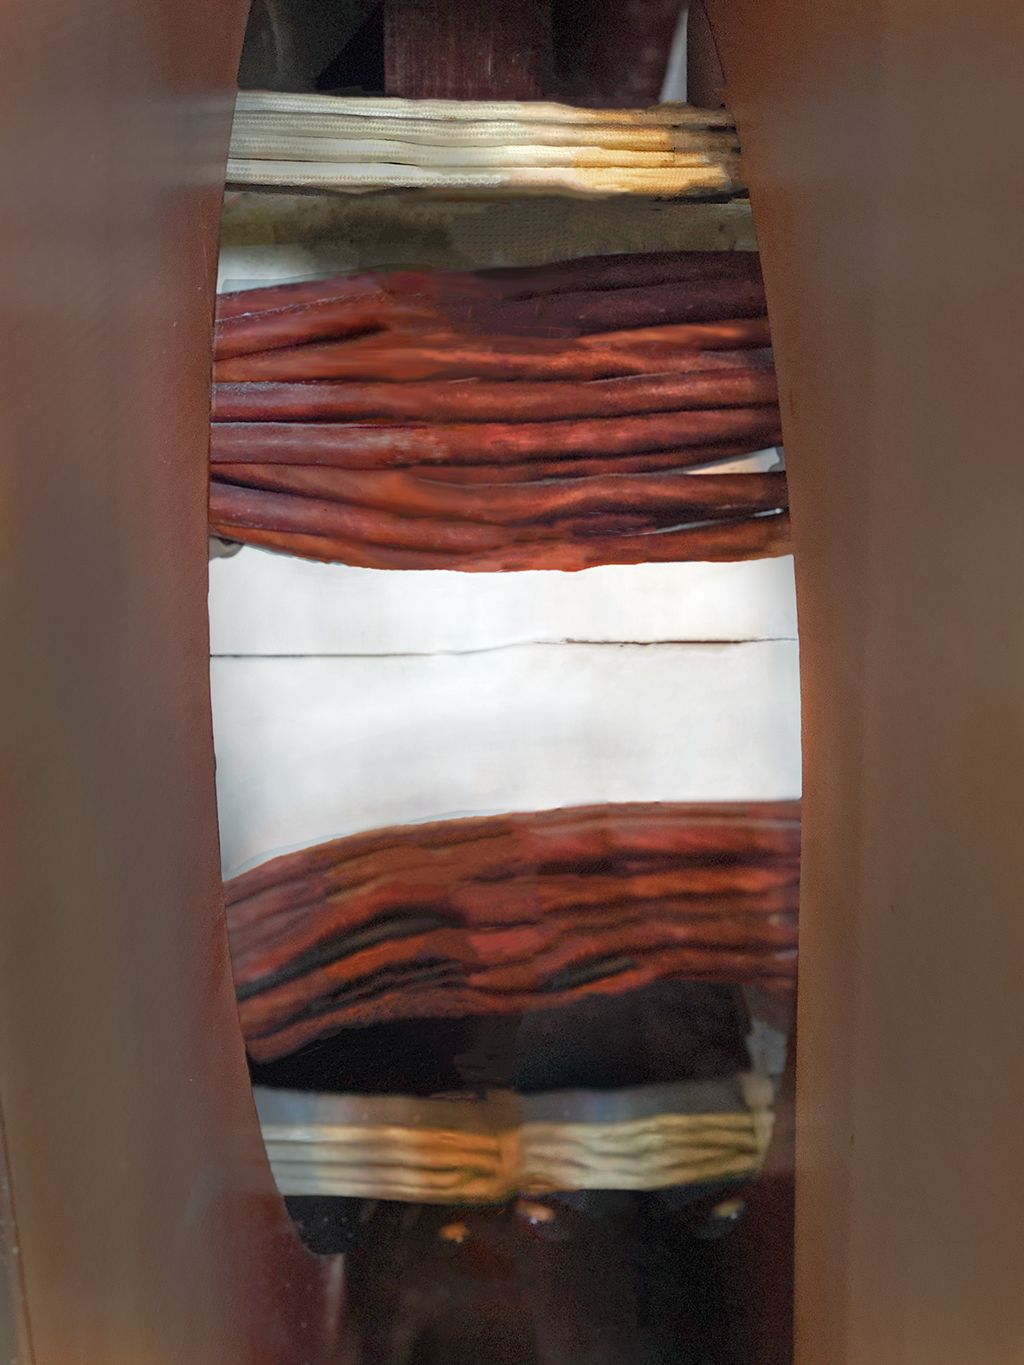
\includegraphics[width=\textwidth]{Chp4/PFCoils.png}
	\caption{\label{ISTTOKpfCoils}PF coils close up,primary coils correspond to the  white cables and vertical and horizontal to the orange ones. }
\end{subfigure}

 \caption{ISTTOK close up side views. \label{ISTTOKviews} }
\end{figure}




\section{ATCA-MIMO-ISOL boards}
\subsection{Hardware layout}
\subsection{Real-time  integration software}
\section{Plasma current magnetic field }

Retrieving the contribution of the plasma current in tokamaks ...

The methods of correction of the magnetic error fields due to inaccuracies
of tokamak manufacturing and assembly are considered. The problems of the
plasma position and shape reconstruction based on magnetic field measurements are discussed.

\section{Plasma centroid position determination}

The vertical and radial plasma position centroid is an essential measurement  since must be computed on real-time so they are the input variables for the ISTTOK control position.
